\chapter{TinyOS and NesC}
\label{ch:tos_and_nesc}

\begin{quotation}
TinyOS is an open source, BSD-licensed operating system designed for low-power wireless devices, such as those used in sensor networks, ubiquitous computing, personal area networks, smart buildings, and smart meters. A worldwide community from academia and industry use, develop, and support the operating system as well as its associated tools, averaging 35,000 downloads a year.

It started as a collaboration between the University of California, Berkeley in co-operation with Intel Research and Crossbow Technology, and has since grown to be an international consortium, the TinyOS Alliance.

{\hfill \cite{TOSnet,TOSw}}
\end{quotation}

TinyOS is written in the NesC programming language, therefore we start with a short introduction to NesC.

\section{The NesC programming language}

Recall traditional C code. In essence it consists of function definitions and variable declarations listed in some order. Calling one function, causes a cascade of other calls, that eventually gets useful work done. Functions providing various aspects of certain functionality or operating on the same data can be grouped together in libraries. Ambiguities start to arise however, when several groups of such functions are mixed together. Moreover, it is not always clear which function should be called and which are considered private.

\subsection{Modules and interfaces}

In \cite{NesC} function grouping is solved more systematically. Each code file must {\bf provide} interfaces, and only through these interface, its functions may be called. An {\bf interface} is nothing more but a set of function names that are implemented in the file that provides it. In the NesC terminology, we call such an interface-enriched file, a {\bf module}.

If interfaces can expose functions to external modules then, by symmetry, there must also be a way to call functions exposed by other external modules. To accomplish that, a NesC module is not only allowed to provide interfaces, but can also {\bf use} them. If the module declares to use an interface, then it's free to call any function this interface contains. At this point, however, it isn't decided where the used interfaces are implemented. The module merely states that it will need them.

To summarize, a module is a C file that provides a set of interfaces and uses a different set of interfaces to help it do the work. This decomposition of an application, that used to be global, into module-sized pieces makes complexity much easier to manage. Moreover, dependencies between pieces and the functionality they require to operate are now explicitly declared, yet the implementation of the functionality can be resolved later. To understand inner workings of a module, one only needs to see its code and the specification of the interfaces it declares to use or provide. No analysis of the interface providers and users is necessary.

\subsection{Configurations}

Pairing a module that uses an interface, with one that provides an implementation of the interface, is done through a new programming construct, called a {\bf configuration}. Configurations, however, do much more than just connecting interfaces of modules together.

Firstly, they can use and provide interfaces just as modules do\footnote{Though only modules contain actual implementations.}. In fact, modules and configurations are so similar than we jointly name them {\bf components}.

Secondly, they can instantiate components. By default all components (modules and configurations) are singletons. If a singleton component isn't ever instantiated in an application, it's omitted during compilation.

Each configuration first instantiates all components it intends to work with. Then it defines connections between their interfaces. Finally, if it has declared to use or provide any interfaces, it passes these interfaces to components it instantiated.  This means that an interface provided by a configuration, may be passed through several layers of configurations until it is finally implemented by some module.

This mechanism forms a basis for creating {\bf self-contained hermetic abstractions}. Precisely, a top-level configuration can provide a set of useful interfaces and hide all their implementation details. The implementation can in turn utilize several layers of abstraction, connect itself to components shared within the application and manage module initialization. However, the user doesn't have to know any of it. All he has to do is instantiating this top-level configuration in his application and making use of the provided interfaces\footnote{In fact, each TinyOS application is such a high-level configuration, that pulls in all dependencies and connects them to the module that implements application logic.}.

We will use a graphical representation of components, as suggested by \cite{Bachmaier} (see Figure \ref{fig:example_component}). Where it's relevant, we'll distinguish modules from configurations by adding \emph{<<realization>>} or \emph{<<specification>>} stereotypes respectively.

\begin{figure}[h]
  \centering
  \includegraphics{diagrams/example_component.eps}
  \caption{Component with one provided and one used interface.}
  \label{fig:example_component}
\end{figure}

\subsection{Two-way interfaces}

NesC interfaces are in fact {\bf two-way}. To explain this concept, we'll consider an example, where a user requests an asynchronous operation. One possible way to support this through interface connections is shown in Figure \ref{fig:two_way_interface1}. User calls \emph{start()} to initiate the operation and \emph{AsyncOpProvider} calls back \emph{completed()} to notify the user about the completion of the operation.

\begin{figure}[h]
  \centering
  \includegraphics[width=0.75\textwidth]{diagrams/two_way_interface1.eps}
  \caption{Asynchronous operation implemented with two interfaces.}
  \label{fig:two_way_interface1}
\end{figure}

Though this scheme works, it forces using two connections where there is only one logical association. The need to connect callbacks, like the \emph{completed()} function in Figure~\ref{fig:two_way_interface1} separately from requests is an unnecessary nuisance. Therefore, NesC allows {\bf events} to be part of interfaces in addition to normal functions, which are known as {\bf commands}. The user of such a two-way interface will have to implement handlers for all events, which again are nothing more than functions with proper names. The scheme, from Figure~\ref{fig:two_way_interface1}, implemented using events is shown in Figure \ref{fig:two_way_interface2}.

\begin{figure}[h]
  \centering
  \includegraphics{diagrams/two_way_interface2.eps}
  \caption{Asynchronous operation implemented with a two-way interface.}
  \label{fig:two_way_interface2}
\end{figure}

\subsection{Parametrized interfaces}
A component may provide a virtualized resource. This means that a real resource is split by software to serve several users. For example, let's consider the problem of waking a group people in a hotel.  Everyone wants to be waken up at different times, but the hotel manager has only a single alarm clock. The solution is simple, the manager has to set the alarm clock for himself, to that of his guests who requested the earliest wakeup time. Then, when the clock rings, he can wake that person up and reset the clock to the next nearest wakeup time, and so on. In essence this scheme crates multiple alarm clocks using only one. We may say that it virtualizes the alarm clock\footnote{This is actually a practical problem in low level programming. Typically, a few hardware timers need to be virtualized, to serve multiple software components.}.

In NesC, this would correspond to providing several \emph{Clock} interfaces, while using only one. Exactly how many of these virtual interfaces should be provided, isn't, however, known ahead of time.  Moreover, if for each virtualized interface, separate function implementations were needed, it would lead to wasteful code duplication.

\begin{figure}[h]
  \centering
  \includegraphics[width=1.0\textwidth]{diagrams/parametrized_interface.eps}
  \caption{Parametrized interface used in timer virtualization.}
  \label{fig:parametrized_interface}
\end{figure}

Instead NesC offers {\bf parametrized interfaces}. They differ from regular interfaces by an additional parameter that their implementing functions receive. This parameter caries the unique identification number of the interface that was used to make the call. It can be treated as a client id.   Notice that this is by far the most convenient way to implement our alarm replicator, because it can use this additional argument to index and update an array of wakeup times and then easily find the earlies one. Sample vitalization of the \emph{Clock} resource is presented in Figure~\ref{fig:parametrized_interface}

\subsection{Generic components}

Implementing a data structure like a bit vector as a singleton doesn't make much sense. Therefore, NesC allows a component to be {\bf generic}. Making a module or configuration generic has two major consequences. Firstly, all its instantiations will create separate and independent components, just as if their code was copied. Secondly, it is possible to pass arguments (both type and value) that will parametrize each such newly created component. Graphically, generic components are distinguished by the parentheses after their name, as shown in Figure~\ref{fig:generic_component}. Note that interfaces
can be type-parametrized as well, which makes generic components a powerful construct.

\begin{figure}[h]
  \centering
  \includegraphics{diagrams/generic_component.eps}
  \caption{A generic component with type and integer arguments,
  providing a parametrized interface.}
  \label{fig:generic_component}
\end{figure}

\subsection{Memory allocation}
Many errors found on wireless sensor nodes, for which software was written in pure C, were caused by various memory related errors. A failed allocation due to a lack of memory and memory leaks were problems particularly painful on nodes with very limited resources.

For this reason, in NesC all memory allocation is static and resolved during compilation. More specifically, each module statically allocates memory for the data on which it operates. This memory is inaccessible to other modules. This way, compiler can easily detect if the required amount of memory exceeds the amount available on the device.

\section{The TinyOS operating system}

TinyOS is written in the NesC programming language. This means, that its made of components which interact with each other only through interfaces. The great advantage of this approach is that these components have clear boundaries and it's easy to understand how to use them. Consider the example shown in Figure~\ref{fig:platform_serial}, which shows the component that gives access to a sensor node's serial port. The port can be used, among others, for communicating with a PC, if the node is connected to the PC with a cable.
\begin{figure}[h]
  \centering
  \includegraphics{diagrams/platform_serial.eps}
  \caption{\emph{PlatformSerialC} gives access to the serial port of the 
           Chronos watch.}
  \label{fig:platform_serial}
\end{figure}
To send data over the port, first you need to call \emph{start()}, then send bytes with \emph{send()} and optionally call \emph{stop()} when serial port is no longer needed. Complex details of handling the hardware are hidden beneath the abstraction. What is important is that this isn't a cleverly chosen example. Components tend to be this intuitive.

Another TinyOS's advantage is its portability. Officially it supports for 22 platforms and many more are available through various project forks. It also comes with many applications that share its core components, most of which are platform independent. The resulting cartesian product of platforms and applications, is incomparably more effective than having applications and platforms tied together.

Testing is also well supported in TinyOS. Firstly, a whole-network simulator (see \cite{TOSSIM}) is available. It allows for simulating the software of not one, but a whole network of nodes, on a PC. Moreover, its radio connectivity models are precise enough to draw reasonably realistic conclusions from the simulations. {\bf TOSSIM} is an invaluable tool for TinyOS developers. Secondly, a NesC unit-testing framework \cite{TOSMock}, has been recently added to TinyOS. {\bf TOSMock}'s ability to verify each component's behavior greatly supplements high-level testing provided by TOSSIM.

Together, these advantages make TinyOS, a good platform for scientific research. TinyOS eases implementation of new algorithms. The richness of existing components, spares the need to implement everything from scratch.  Moreover, existing components tend to be well tested, which minimizes the chance of programming errors.  Multitude of supported platforms make it easy for different groups to use the same software on their varying hardware.  Comparison of results is also much easier thanks to the use of a common system.  Researchers can easily run competitive solutions side-by-site to learn their flaws and find ways to improve them.  Particularly, in networking research, it's much easier to experiment with a single element of the network stack, when the rest of the stack is available and tested. It is possible to do incremental improvements, which is the essence of scientific development.

\subsection{Anatomy of an application}

In this section, we explore a simple TinyOS application and explain how it works. Its purpose is to periodically blink a Light-Emitting Diode (LED). The root of the application is a configuration named \emph{BlinkAppC}\footnote{By convention, letter \emph{P}, at the end of a component's name means that the components is private, while \emph{C} the component as marks a useful public abstraction.}. The logic is in turn implemented in module \emph{BlinkC}. The module uses three interfaces to achieve its goals. Firstly, it needs an entry point. This is provided by the \emph{Boot} interface that signals an event, \emph{booted()}, after system initialization is complete.  Secondly, the LED is controlled through the \emph{Leds} interface. Finally, timing is managed with the help of the \emph{Timer<TMilli>}\footnote{\emph{TMilli} serves to distinguish timers with different resolution.} interface. The entire structure of the application is shown in Figure~\ref{fig:app_anatomy}.  The \emph{booted()} event implementation configures the timer to repeatedly send the \emph{fired()} event. The implementation of the event, in turn, toggles the state of the LED. This logic is reflected in the following code:

\begin{lstlisting}[numbers=none, keywordstyle=\bfseries, language=C]
  event void Boot.booted()
  {
    call Timer.startPeriodic(250);
  }
  event void Timer.fired()
  {
    call Leds.led0Toggle();
  }
\end{lstlisting}

\begin{figure}[h]
  \centering
  \includegraphics[width=1.01\textwidth]{diagrams/app_anatomy.eps}
  \caption{Structure of the Blink application.}
  \label{fig:app_anatomy}
\end{figure}

Interfaces, used by Blink, are implemented by three distinct components.  The \emph{LedC} configuration, which provides the Leds interface, is part of the by TinyOS library.  As shown in Figure~\ref{fig:ledc}, it uses a platform-specific component \emph{PlatformLedsC}, which simply gives access to the MCU IO pins to which LEDs are connected. Most platforms supported by TinyOS provide this component\footnote{Though, some platforms provide fewer leds, replacing missing ones with stubs. Chronos watch, having no LEDs, uses it's LCD display.}.
\begin{figure}[h]
  \centering
  \includegraphics[width=0.8\textwidth]{diagrams/ledsc.eps}
  \caption{The \emph{LedsC} configuration.}
  \label{fig:ledc}
\end{figure}

This pattern is quite common. Often, platform independent logic is implemented in the library. To support such a library, the platform must implement certain lower-level components.  If it doesn't, an attempt to use the library causes a compilation error.

The timer library requires the \emph{HilTimerMilliC} component, but this is explained in the next section. \emph{MainC} is related to the system initialization sequence. Therefore, a task scheduler must be introduced before we look into it.

\subsection{Timer subsystem}
\label{ch:timer_subsystem}

The generic configuration \emph{TimerMilliC()} serves one purpose. It provides a single instance of the \emph{Timer<TMilli>} interface and internally connects it to the component that virtualizes the timers, thorough a parametrized interface. In this way, the user doesn't have to figure out the parameters himself\footnote{The details of how these parameters are handled are explained in \cite[ch. 6]{TOSProg}.}.  Figure~\ref{fig:timermillic} shows that the interface is connected to component \emph{TimerMilliP}.
\begin{figure}[h]
  \centering
  \includegraphics{diagrams/timermillic.eps}
  \caption{The generic \emph{TimerMilliC} configuration.}
  \label{fig:timermillic}
\end{figure}
\emph{TimerMilliP} is a singleton supporting all instances of \emph{TimerMilliC}. Its structure is presented in Figure~\ref{fig:timermillip}.
\begin{figure}[h]
  \centering
  \includegraphics{diagrams/timermillip.eps}
  \caption{The singleton \emph{TimerMilliP} configuration.}
  \label{fig:timermillip}
\end{figure}
For the initialization, it relies on \emph{MainC}. The timers are in turn virtualized by a third component called \emph{HilTimerMilliC}\footnote{HIL stands for Hardware Independence Layer and is explained in section \ref{haa_arch}.}. This last component is provided by the platform, though in its implementation many library components are used.

\subsection{Tasks and the task scheduler}

Applications need to perform multiple operations simultaneously. As sensor nodes typically have too little memory to support fully fledged threads, another solution is needed. Therefore, NesC cooperates with TinyOS to provide {\bf task management}. A task is simply a parameterless function with no return value. Tasks are used to split all lengthy operations into smaller portions that can be interleaved with each other, giving the impression of parallel execution. It's important to keep tasks short; otherwise, the latency of the system may be reduced, for example, when tasks of short operations wait for a single long one.

Only one task runs at any given instant and it cannot be preempted by another task. Moreover, the task will run only once regardless of the number of times that it has been posted for execution. A single bit is preallocated to mark the task as posted and ready for execution.

The execution is handled by the \emph{TinySchedulerC} component, depicted in Figure~\ref{fig:tinyschedulerc}\footnote{The meaning of the \emph{async} keyword is explained in Section \ref{sec:interrupts_and_async}.}. This component is also used by the NesC compiler to generate task related code. Exactly, what happens behind the scenes is that when a component declares a task it actually provides a hidden \emph{TaskBasic} interface, corresponding to the task. The interface allows the component to post the task to the scheduler and contains an event signaled whenever the scheduler selects the tack for execution.  All \emph{TaskBasic} interfaces are connected to the \emph{SchedulerBasicP} module that handles their queueing and also contains the main task loop.

The \emph{McuSleep} interface is used when the main task loop has been started but there are no tasks pending. In such a case, MCU enters the lowest safe sleep state\footnote{The sleep level depends on the peripherals left running. Not all can operate in the lowest power mode.} with the McuSleep interface.

\begin{figure}[h]
  \centering
  \includegraphics[width=1.02\textwidth]{diagrams/tinyschedulerc.eps}
  \caption{The TinyOS's task scheduler structure.}
  \label{fig:tinyschedulerc}
\end{figure}

\subsection{\emph{MainC} configuration and system initialization}

The \emph{MainC} component is special it two ways. Firstly, it contains the entry point to the entire TinyOS code, because it implements the \emph{main()} function. It says a lot about NesC, that it abstract something like the \emph{main()} function with a component. Secondly, \emph{MainC} handles whole initialization sequence of TinyOS and the hardware platform. The diagram of its structure is shown in Figure~\ref{fig:mainc}.
\begin{figure}[h]
  \centering
  \includegraphics[width=0.98\textwidth]{diagrams/mainc.eps}
  \caption{Structure of the \emph{MainC} configuration.}
  \label{fig:mainc}
\end{figure}

The \emph{PlatformC} component is the top-level abstraction for the underlying platform. Its responsibility is to initialize the hardware. This is done when \emph{RealMainP}, which contains the implementation of the \emph{main()} function, calls the \emph{PlatformInit} interface. The TinyOS {\bf initialization sequence} consists of the following steps:
\begin{enumerate}
  \item The global function \emph{platform\_bootstrap()} is called to do any platform specific initialization that cannot wait, such as disabling a watchdog\footnote{Watchdog is a recovery subsystem, that resets the device in case of a software failure, like a deadlock.} timer.
  \item The scheduler is initialized through the \emph{Scheduler} interface.
  \item The hardware platform is initialized through the \emph{PlatformInit} interface.
  \item Any tasks posted during the platform initialization are run until completion.
  \item The software components are initialized through the \emph{SoftwareInit} interface.
  \item Any tasks posted during the software initialization are run until completion.
  \item When both the hardware and the software are ready, hardware interrupts are enabled.
  \item The \emph{booted()} function of the \emph{Boot} interface is called.
  \item The task scheduler enters the main task loop.
\end{enumerate}
All other software components connect their initialization to the \emph{SoftwareInit} interface of \emph{MainC}. This helps avoid omitted or double initialization errors.

\subsection{Interrupt handling and asynchronous events}
\label{sec:interrupts_and_async}

Hardware often needs to notify software that a certain event occurred. This could be, among others, a reception of a radio packet or an arrival of a temperature measurement. Sending such a notification is possible through a mechanism of so-called {\bf interrupts}. When an interrupt occurs, the processor immediately stops executing instructions and jumps to a special interrupt handler function\footnote{TinyOS allows to implement the interrupt handlers with the \emph{TOSH\_SIGNAL()} macro.}. After it returns, execution resumes from where it was interrupted.

The fact that interrupts can fire at arbitrary moments causes serious concurrency problems. They can and often do occur in the middle of some task being executed.  Consider the following scenario. A task is copying bytes from a queue. Then a radio packet arrives and an interrupt fires. The handler adds this packet to the queue. Suppose that the task resumes execution, and is unaware of the interrupt. It thus may overwrite the queue state variables with stale values. In effect, the received packet may be lost and the queue may end up in an invalid state.

Interrupts can be made to wait for the current task to finish.  Alternatively, each interrupt could post a special task to the scheduler. Neither of these is good choice though, because most interrupts are time-critical. For example, an interrupt might inform the MCU that a new byte was received from a communication bus. This byte must then be read from the input register, before another received byte replaces it. In such cases, delays may lead to subtle run time errors.

NesC and TinyOS solve these concurrency problems by dividing the code into two parts: synchronous code (SC) and asynchronous code (AC).  All code reachable from interrupt handlers is considered to be AC. An implementation is considered safe, if {\bf each variable is either only accessed from SC or every access to it is protected with an \emph{atomic} block}. Tasks, by definition are SC. Commands and events, that are not SC have to be marked with the \emph{async} keyword. In particular, its use shown in Figure~\ref{fig:tinyschedulerc} means that tasks can be posted from AC. The clear separation of interrupt handling from the task execution, reduces the chances of errors and makes code more readable. Moreover, the NesC compiler verifies the above constraints and issues warnings if potential race conditions are detected. For more information, refer to \cite[ch. 8]{NesCMan}.

\subsection{The TinyOS component organization structure}

TinyOS components are organized based on their function, hardware
dependence and re-usability. In this section, we list the most
important categories present in the system.

\begin{itemize}
  \item {\bf Global interfaces} connect many important and independent components. Among them are the definitions of \emph{Read}, \emph{Write}, \emph{Send}, \emph{Boot} and \emph{Init} interfaces. They are located under the \emph{tos/interfaces/} path.

  \item {\bf Libraries} contain relatively hardware-independent code.  This means, for instance, that a MAC layer library may assume that a radio chip operates on packets, rather than byte streams, but it will not assume any particular chip family. Libraries are located under \emph{tos/lib/}, \emph{tos/system/} paths. The first path typically contains various protocols and algorithm implementations. The second contains components that are integral parts of TinyOS or are heavily shared among platforms, such as the scheduler, the \emph{LedsC} and \emph{MainC} configurations.

  \item {\bf Chip drivers} contain components that are meant to operate particular hardware chips. They are located under the \emph{tos/chips/} path. For example, one of the drivers is called \emph{at45db} and supports an external flash memory chip of the same name. Any platform, that makes use of this chip can also use this driver. In hardware design, chips are abstractions that hide their internal workings. The same is true for their drivers. Often, it's only necessary to make a few component connections that represent physical connections on the circuit board to incorporate a driver into a platform.

  \item {\bf Platforms} contain sets of components needed to support particular circuit boards. They are located under \emph{tos/platforms/}. One notable example is the \emph{chronos} platform, which is the subject of this work. A special file, named \emph{.platform}, holds the configuration parameters for the compiler. Among others, it lists platform dependencies and the MCU the compiler should generate code for. A platform directory  also contains the \emph{PlatformC} component, which is the main entry point to hardware initialization code, along with many other hardware dependent components that enable various functions and features.

  \item {\bf Applications} are located under the \emph{apps/} path. Each consists of a root configuration, helper components, a \emph{Makefile} and a \emph{README} file. The \emph{Makefile} guides the build process\footnote{It's worth to note, that usually nowhere in an application is any particular platform specified. Instead, every application can be built for any platform, which is selected by an argument to the \emph{make} command.} and the \emph{README} contains useful comments on the application operation.

  \item {\bf Support build rules} are located under the \emph{support/make/} path. They define exactly how the build process for each platform should progress.

\end{itemize}

\subsection{The Hardware Abstraction Architecture (HAA)}
\label{haa_arch}

TinyOS employs a so-called {\bf Hardware Abstraction Architecture}, whose idea arises from the desire for the hardware related code to the have the following three properties. Firstly, we would like the low-level code to be clear and readable. Code that, for example, makes uncommented register accesses is difficult to maintain in the long run. Such bad practices also cause many programming errors, yet they are tempting. Secondly, we would like to have useful abstractions of all available hardware features. Often, they allow for making important performance optimizations. Access to hardware should, however, be made at a relatively high level, which prevents errors caused by forgetting certain details related to the hardware's operation. Such details should be taken care of behind the scenes. Thirdly, we would like to have certain abstractions that are hardware independent. A notable example is radio networking, where we want an interface that allows us to communicate regardless of the radio chip used. Often, conforming to such interface requires implementing some of its functions in software, while ignoring some other features that the hardware provides. To meet these goals, TinyOS proposes splitting the code according to a three-layer architecture \cite{TEP2} depicted in Figure~\ref{fig:haa_diagram}.
\begin{figure}[h]
  \linespread{0}
  \begin{verbatim}
                           +-----------------------------+
                           |                             |
                           | Cross-platform applications |
                           |                             |
                           +--------------+--------------+
 +-----------------+                      |                  +-----------------+
 |Platform-specific|                      |                  |Platform-specific|
 |  applications   |                      |                  |  applications   |
 +--------+--------+                      |                  +--------+--------+
          |          Platform-independent | hardware interface        |
          |        +-------------+--------+----+-------------+        |
          |        |             |             |             |        |
          |  +-----+-----+ +-----+-----+ +-----+-----+ +-----+-----+  |
          |  |.----+----.| |.----+----.| |.----+----.| |.----+----.|  |
          |  ||         || ||         || ||         || ||  HIL 4  ||  |
          |  ||  HIL 1  || ||  HIL 2  || ||  HIL 3  || |`----+----'|  |
          |  ||         || |`----+----'| |`----+----'| |     |     |  |
          |  |`----+----'| |     |     | |     |     | |     |  +--+--+
          +--+--+  |     | |.----+----.| |     |     | |     |  |  |
             |  |  |     | ||         || |.----+----.| |.----+--+-.|
             |.-+--+----.| ||         || ||         || ||         ||
             ||         || ||  HAL 2  || ||         || ||         ||
             ||         || ||         || ||  HAL 3  || ||  HAL 4  ||
             ||  HAL 1  || |`----+----'| ||         || ||         ||
             ||         || |     |     | ||         || ||         ||
             ||         || |     |     | |`----+----'| |`----+----'|
             |`----+----'| |.----+----.| |     |     | |     |     |
             |     |     | ||         || |.----+----.| |     |     |
             |.----+----.| ||  HPL 2  || ||         || |.----+----.|
             ||  HPL 1  || ||         || ||  HPL 3  || ||  HPL 4  ||
             |`----+----'| |`----+----'| |`----+----'| |`----+----'|
             +-----+-----+ +-----+-----+ +-----+-----+ +-----+-----+  HW/SW
                   |             |             |             |          boundary
        ************************************************************************
            +------+-----+ +-----+-----+ +-----+-----+ +-----+-----+
            |HW Plat 1   | |HW Plat 2  | |HW Plat 3  | |HW Plat 4  |
            +------------+ +-----------+ +-----------+ +-----------+
  \end{verbatim}
  \centering
  \caption{The Hardware Abstraction Architecture (source \cite{TEP2}).}
  \label{fig:haa_diagram}
\end{figure}
Each layer is founded on top of the previous one, hardware being at the bottom and hardware independent applications at the top.

Right above the hardware lies the {\bf Hardware Presentation Layer (HPL)}. Its purpose is to hide (often crude) ways in which hardware is accessed behind NesC interfaces. It's possible for several components to form the HPL layer. For example, register access can be handled better if register reading and writing is separated from the meaning of these operations. However, these components should have no state, no logic and only precisely present commands that can be sent to the hardware and translate interrupts so that they appear as asynchronous events. The rationale for this is that we want to keep HPL components as simple as possible, because hardware access makes them already complex enough.

The {\bf Hardware Abstraction Layer} is made of components that implement all the logic for handling the hardware. They access the hardware through HPL and provide abstract, easy-to-use interfaces for applications and the HIL layer. HAL components can have state and should use it to hide the burden and subtleties related to hardware operation. On the one hand, they should ease the application development, and on the other, allow for fully utilising the hardware, to achieve a maximum application performance.

By its nature, HAL is hardware dependent. Therefore, on top of it, the {\bf Hardware Independence Layer} is introduced. It should provide a set of well defined\footnote{Most HIL interfaces are described in TinyOS Extension Proposals.} interfaces, which are designed for hardware independence. Often, there is a discrepancy between hardware features and what is required to meet the interface.  Designers try to shorten this gap by distilling a common subset of functions typically available in most types of hardware. Still there may be need to either virtualize the resource or provide some kind of access arbitration to hide its singleton nature and provide other features through software algorithms.

Typically, a developer should first try to use only HIL interfaces in his application and only, if considerable performance gains are possible, should he resort to using HAL interfaces. In this way, a maximum hardware independence is assured.

\subsection{Integrated power management and concurrency control}
\label{ch:concurrency_and_power}

Power management is critical in sensor network applications, which usually rely on battery-powered nodes. One aspect of this is related to peripheral devices: external chips, MCU subsystems and data buses. They need to be powered down whenever not in use. For this, approach exact information about the device usage is needed.  Getting such information is tricky, however, especially when multiple clients compete for access to the device, in which case the access has to be arbitrated to avoid collisions.  This leads to the conclusion that joining concurrency control and power management may be beneficial. Knowing the concurrency, we can share the device among clients and also power it down when it's not in use.

\cite{Klues et al.} proposes an elegant design that allows to implement this idea in TinyOS. We will present it in the following example, which closely resembles real applications.

Assume that a node contains a certain hardware device. This device can perform several functions, but only one can be selected at a time and only one user can use the device at any time. Moreover, it is necessary to power down the device once its current function has been deactivated. There are several clients wishing to use the device and each knows ahead of time which function it will be interested in.
\begin{figure}[h]
  \centering
  \includegraphics[width=1.0\textwidth]{diagrams/devicearbiterp.eps}
  \caption{Component that arbitrates access to the device and powers
  it down when not in use.}
  \label{fig:devicearbiterp}
\end{figure}

\begin{figure}[h]
  \centering
  \includegraphics[width=1.0\textwidth]{diagrams/devicefunction1c.eps}
  \caption{Generic configuration that client uses to access the
  the device.}
  \label{fig:devicefunction1}
\end{figure}
The proposed solution consists of two abstractions (see Figure~\ref{fig:devicearbiterp} and \ref{fig:devicefunction1}). Arbitration between the clients is handled by \emph{DeviceArbiterP}, which uses a system library component named \emph{FcfsArbiterC}. The first-come-first-server arbiter queues requests for device access and grants it to each subsequent client in turn. It also takes care of configuring the device for each client before granting the access. Finally, when there are no more pending requests, it leaves the device to its default owner - the \emph{DevicePowerDownP}. This power manager, turns the device off upon acquisition and  on when it's requested again by the arbiter. Users do not access \emph{DeviceArbiterP} directly, but rather use a series of generic function access components. One of them is shown in Figure~\ref{fig:devicefunction1}.
A client wanting to use the first function of the device creates an instance of this configuration, which gives him \emph{Resource} and \emph{DeviceFunction1} interfaces. The first one must be used to secure access to the device.  Then, the second one allows for actually using the device.  Note that in NesC it's possible to wire twice to the same interface.  \emph{DeviceFunction1P} uses this feature to assert that device access was really acquired by the user.

\subsection{Conclusion}
TinyOS is an advanced sensor node operating system. It solves many issues, plaguing traditional development of software for battery powered devices and provides a solid foundation for advanced applications and algorithms. As Chronos is part of the family of devices that TinyOS was designed to support, we believe that bringing it to the watch, will open a multitude of paths for further platform development.

% To enable wrapped line navigation:
% map j gj
% map k gk

% Vim settings:
% vim: set nonumber:
% vim: set spell:
% vim: set linebreak:
% vim: set wrap:
% vim: set textwidth=0:
% vim: set fo+=t:

